%  LP: la partie commentee ci-dessous a ete copié dans le fichierA
%  ``reference_flux.tex'' (peut etre supprimee ici)

%\subsubsection{Reference flux densities of secondary calibrators}
%\label{se:fluxSec}
%(revised by JFL Aug 2017 - must remove the old version in photometry-HA.tex)
%

%++ SPIRE refer.


\subsection{Aperture photometry}
\label{S:ApPh}

Generally speaking, 
photometry is most advantageously done by PSF fitting when  target is a point-source and the telescope PSF is well known.
The 30-metre PSF with NIKA2 is not fully caracterised yet and likely depend on elevation and atmospheric conditions.
Hence, instead of PSF fitting, we have used aperture photometry to
recover as much as possible of the calibrator flux spread over the main beam and side
lobes of the telescope for our study of the stability of the calibration. 
For this study, observations were beammaps and $8' \times 5'$ otf's of the primary calibrators Uranus and Neptune
and of the secondary calibrators MWC349A, NGC7027 and CRL2688. All are
point-sources or quasi, except NGC7027 which is slightly extended.

We describe now how we have implemented aperture photometry.

All observations (beammaps and $8' \times 5'$ otf's) were first processed 
with the pipeline set up with the parameters of Table~\ref{tab:Pipe} to produce the intensity map of each array.
We stress that the  gain-elevation curve of EMIR implemented in the pipeline was NOT  turned on for this processing.

\begin{table}[h]
\begin{center}
\begin{tabular}{|l|c|c|}
\hline
                      &    run 9                             &  run  10                   \\
\hline
kidpar                &  {\scriptsize kidpar-best3files-FXDC0C1-GaussPhot} &  {\scriptsize kidpar-n2r10-calib.fits}   \\
Decorrelation method  &  {\scriptsize COMMON-MODE-ONE-BLOCK} &    {\scriptsize COMMON-MODE-ONE-BLOCK}    \\
Opacity               &  {\scriptsize  l.o.s}                &  {\scriptsize l.o.s}     \\
Sky Projection        &  {\scriptsize RADEC}                  &  {\scriptsize RADEC}     \\
a priori mask         &  {\scriptsize   $50''$}              &  {\scriptsize $100''$}  \\
Iteration in mapping  &  {\scriptsize  None}                 &  {\scriptsize None}     \\
Elevation gain curve  &  {\scriptsize  None}                 &  {\scriptsize None}      \\
\hline
\end{tabular}
\caption[]{Pipeline set-up for processing of the calibrators.}
\label{tab:Pipe}
\end{center}
\end{table}

The total flux density of a source  measured over an aperture  is :

\begin{equation}
S_{\nu} = \sum_{m} \sum_{n}  I_{m,n} ({\rm Jy/beam}) \times {dx^2 \over {\Omega_{true}}}
\label{eq:ApPh}
\end{equation}


\noindent  $I_{m,n}$ is the brightness in Jy/beam measured in each
pixel $(m,n)$ of the NIKA2 map ; $dx$ is the pixel size ;
$\Omega_{true}$ is the solid angle of the total beam named $true$ by usage ; pixel
indices $m,n$ are such that $dx \times \sqrt{(m-m_c)^2 + (n-n_c)^2} < 150''$ with 
$m_c,n_c$ being the map center., i.e. radial distance is smaller than the aperture radius $150''$.

In each pixel, brightness $I_{m,n}$ is naturally expressed in unit of
Jy/beam where  {\it beam } stands for the total beam of the telescope. This is because the
source power incident on the telescope is captured both through its main
beam and side lobes, {\it i.e.} through its total beam.
Hence, prior to summing all pixels within the aperture, brightness $I_{m,n}$ 
must be converted from natural unit Jy/beam to Jy/pixel. This
conversation is done with the factor $dx^2 \over {\Omega_{true}}$ 
which  is, effectively, {\bf the pixel area $dx^2$  in unit of fractional beam}
\footnote{(--check this--) in the pipeline, aperture photometry assumes the solid angle of a fixed Gaussian beam, and so :
  $$S_{\nu} = \sum_{m} \sum_{n}  I_{m,n} ({\rm Jy/beam}) \times {dx^2 \over {2 \pi \sigma_0^2}}$$
  where the conversion factor becomes ${dx^2 \over {2 \pi \sigma_0^2}}$, with
  $\sigma_0=FWHM0/2\sqrt{2 ln2}$ for the Gaussian FWHM0=$12.5''$
and $18.5''$ at 1 and 2 mm, respectively.  Note that ${\Omega_{true}} \over {2 \pi \sigma_0^2 }$  is $\sim$~1.5 and $\sim$~1.2 at 1 and 2 mm, respectively.}.
Pratically, $dx^2$ being set in arcsec$^2$ in the pipeline,
$\Omega_{true}$ must  be measured in arcsec$^2$ also.

The computation of the solid angle of the total beam $\Omega_{true}$ depends on the
observation frequency $\nu$ and on the radius $r_{max }$ allowed by the
map size. It can be measured as :

\begin{equation}
 \Omega_{true} (\nu,r_{max}) = \int_0^{2\pi} \int_0^{r_{max}} B(\nu, r) 2 \pi r dr
\label{eq:Otrue}
\end{equation}

\noindent where $B(\nu,r)$ is the radial profile of the source obtained in azimuthally averaging brigthness over narrow annuli
$dr$ in width, and normalised so that B(0)=1 (R. Adam's thesis (2016) or J.D. Kraus (1980)).
(Equally valid is the  direct summation of the pixels in each annuli scaled  appropriately so that B(0)=1). 
We have used $r_{max}=250''$ which is the maximum extent allowed by
the size of the maps acquired during observations of runs 9 and 10.
Power left beyond $r_{max}=250''$ at 260 GHz is between 34\%, as
estimated at 280 GHz, and 21\% at
210 GHz in using parameters in Tables 1 and 4 of Kramer et al
(2013) (amplitudes of the three error beams, $\eta_{fss}$ and 1-Feff and see Carsten's email).

The excess of the total beam relative to the Gaussian beam is the ratio
$\Omega_{true} / 2 \pi (\sigma_{Gauss})^2$, with  $\sigma_{Gauss}$ derived from the $FWHM$ determined
with  the NIKA2 map for a point-like source.


\subsection{Determination of the solid angle of the total beam with Uranus and Neptune : }
\label{S:solang}


The solid angle $\Omega_{true}$ of the total beam has been computed with  eq.~\ref{eq:Otrue}
as well as its excess relative to the Gaussian main beam 
for each  observation of Uranus and Neptune in  runs 9 and 10 under a broad range of atmospheric conditions
($0.05 < \tau_{1mm} < 0.65$)  and histograms of their values are shown in Fig. ~\ref{fig:Otrue}.

\begin{figure}[th]
\begin{center}
  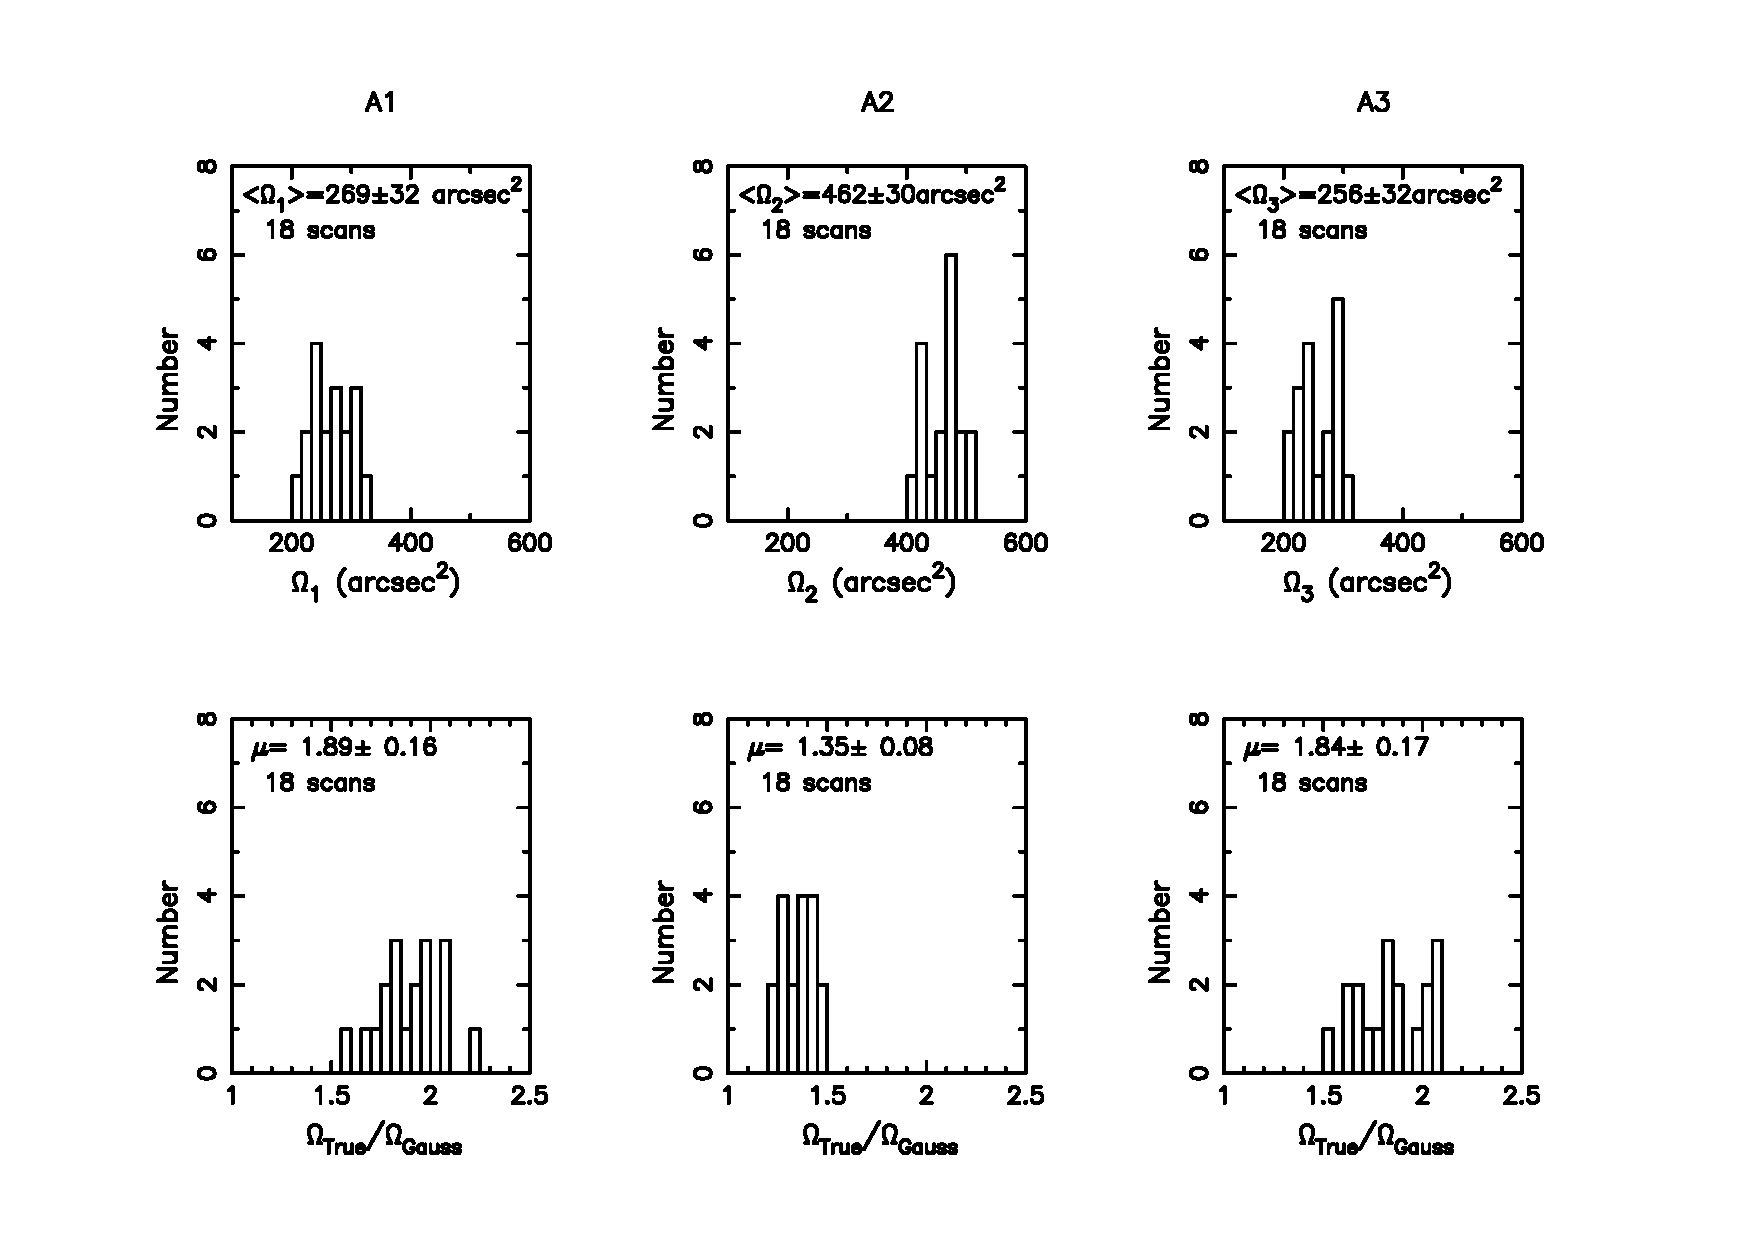
\includegraphics[clip, angle=0, scale=0.6]{Figures/Hist_omega_true_and_excess.pdf}
  \caption{Top line : solid angles of the total beam
    ($\Omega_{true}$) for arrays A1, A2, A3. Bottom line :  excesses relative to the Gaussian main beam
   ($\Omega_{true} / 2 \pi (\sigma_{Gauss})^2$ for the three
   arrays. All 18 observations of Uranus and Neptune a
   during runs 9 and 10 are shown ($\sigma_{Gauss}$ is related to the FWHM actually measured for the
   Gaussian main beam for each observation, i.e. it is not related to the reference FWHM0 $12.5''$ and $18.5''$).
   Mean and rms are provided for the three arrays. {\bf FM: the scale of the
     y axis should be much smaller ; JFL : will be done for final
    version of document}}
\label{fig:Otrue}
\end{center}
\end{figure}

We have found that the solid angle of the total beam is slightly variable and its mean and rms are
$269\pm32$, $462\pm30$, and $256\pm32$ arcsec$^2$ for arrays 1, 2, and
3, respectively. We note 
that $\Omega_{true}$ is proportional to $\nu^{-1}$ as expected. The excesses of the total beam
relative to the Gaussian main beam (ratio of solid angles) have means and rms
of $1.89\pm0.16$, $1.35\pm0.08$ and $1.84\pm0.17$, for arrays 1, 2 and 3, respectively.
The beam efficiencies (ratio of powers between main beam  and total
beam) can be derived in inverting these ratios. These efficiencies are
$\sim 55$ \% at 1mm ($(1/1.87) \times 100$) and $\sim 70$ \% at 2mm ($(1/1.35) \times 100$)
over the extent $r_{max}=250''$ and are consistent with the direct
determination reported in Table~\ref{tab:beam_efficiency} in \S~\ref{se:beams}.
 
\noindent {\bf FM: it would help the reader to have all these values
  in a table ; JFL's reply at the moment : inconsistencies between numbers in Table~\ref{tab:beam_efficiency}
  above required some discussion. }\\ 
 
 
We have searched for any systematics in  $\Omega_{true}$ with respect to elevation,
opacity,  and transmission ($exp(-\tau/sin(elev)$) in Fig.~\ref{fig:Osystematics}.
Over the limited range of elevations between  33$^{\circ}$ and 58$^{\circ}$ covered by these observations,
there is no definitive correlation although
a 15\% increase of $\Omega_{true}$ at small opacity ($<0.15$) and, consequently,
at high transmission ($> 0.8$), is hinted by inspection of the plots.
This effect is not understood and under investigation. 

\begin{figure}[p]
\begin{center}
  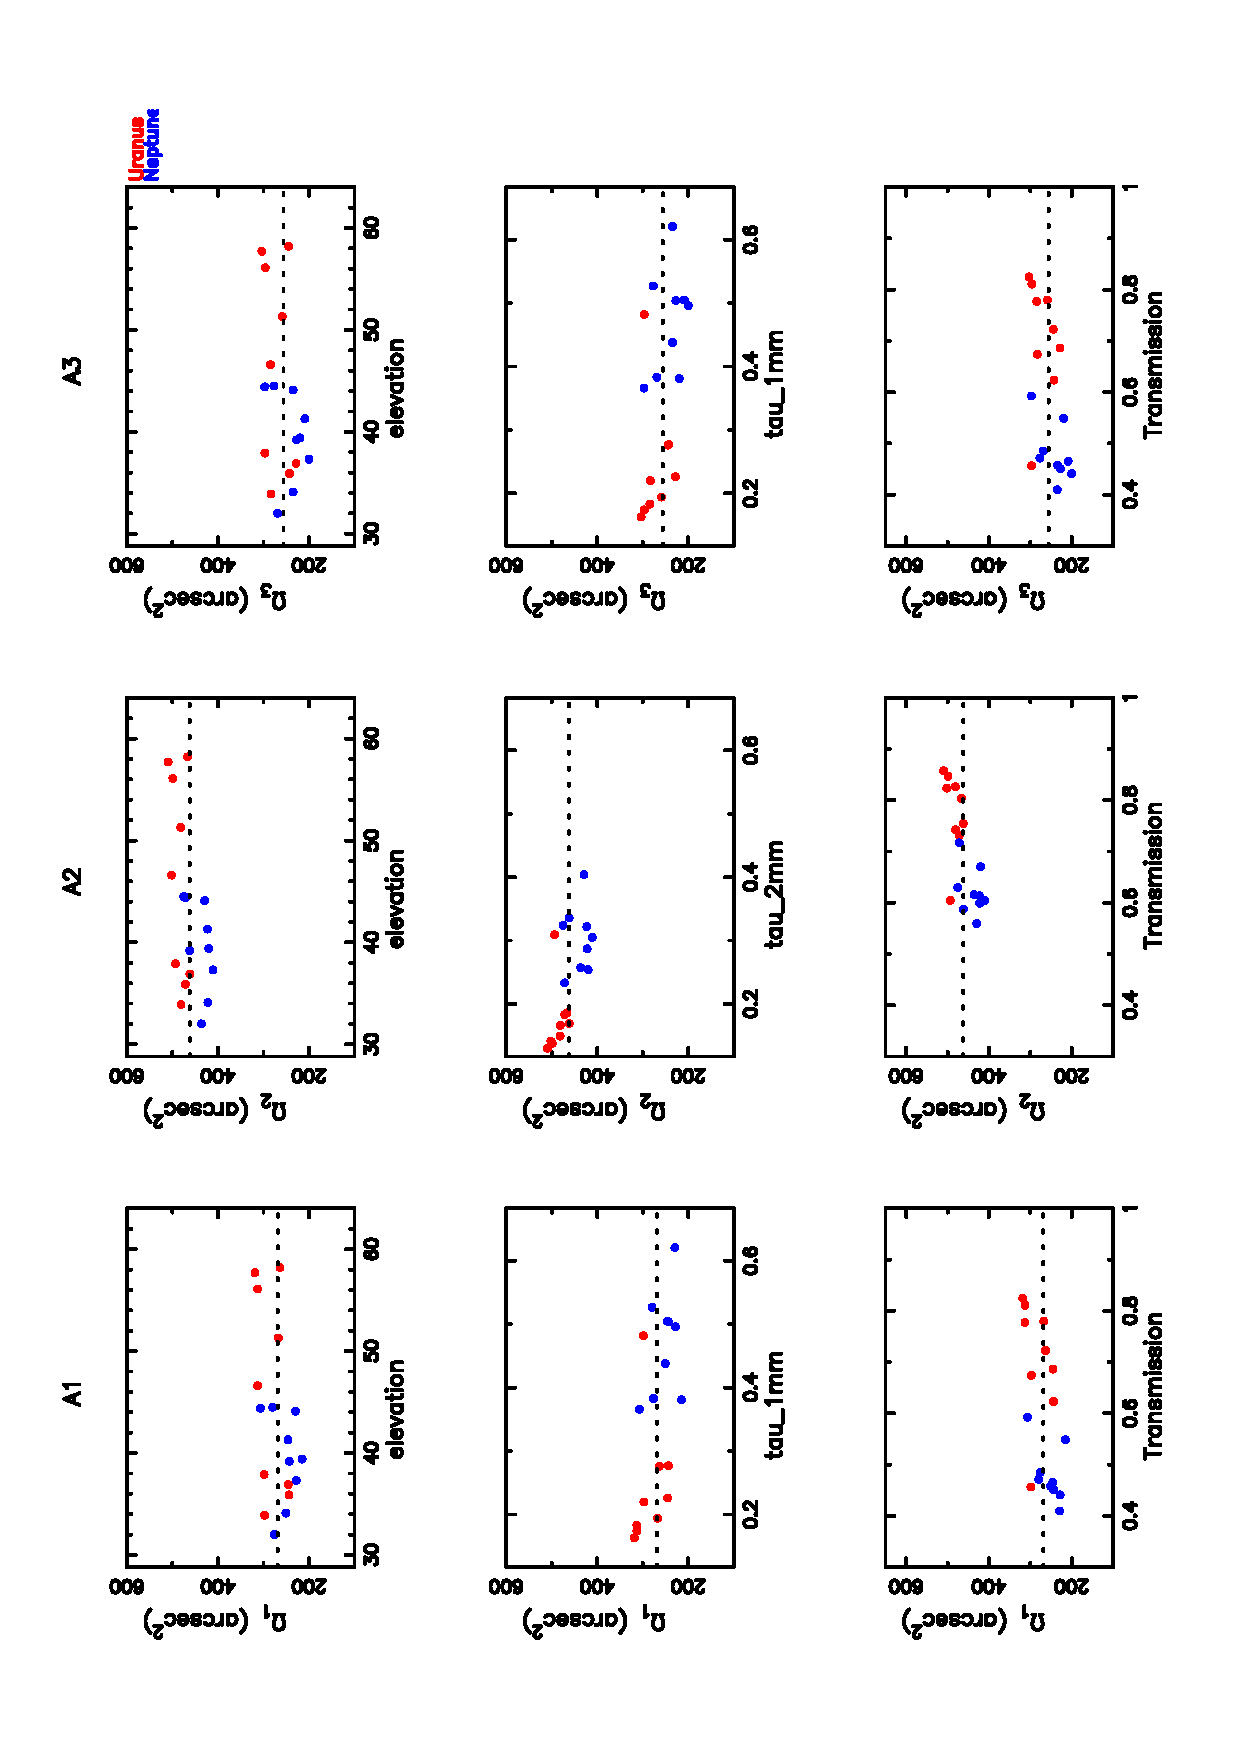
\includegraphics[clip, angle=-90, scale=0.6]{Figures/Omega_True_vs_elev_tau_transmission.pdf}
  \caption{Search for systematics in the solid angle of the total beam $\Omega_{true}$
   with respect to elevation, opacity and transmission
   ($exp(-\tau/sin({\rm elev})$) of all 18 observations
   of Uranus and Neptune during runs 9 and 10. There is no definitive correlation although a 15\% increase
   of $\Omega_{true}$ at small opacity ($<~0.15$), and consequently
  at high transmission ($>~0.8$), is hinted by close inspection of these plots. {\bf FM: the scale of the
    y axis should be much shorter ; JFL's reply : will be done for final
    version of document}}
\label{fig:Osystematics}
\end{center}
\end{figure}


\begin{figure}[p]
\begin{center}
  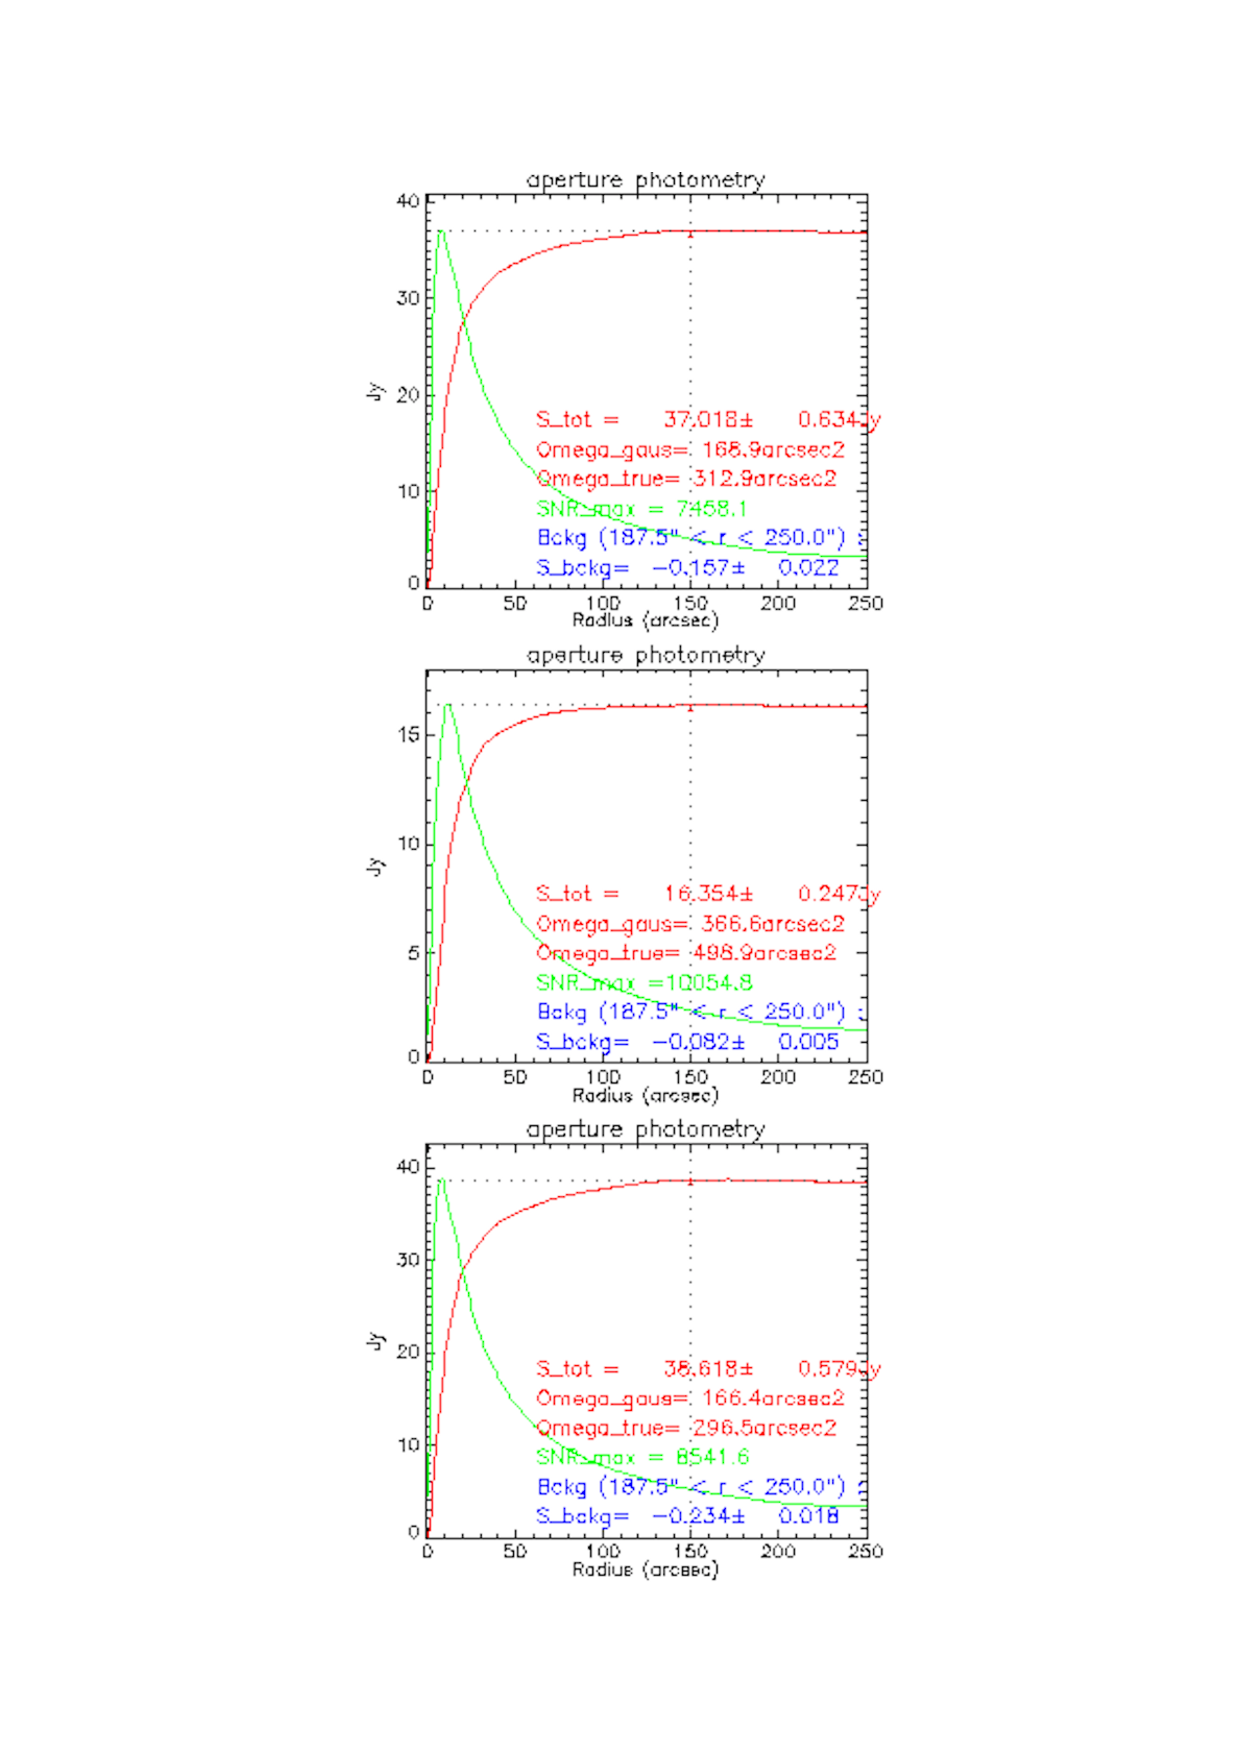
\includegraphics[clip, angle=0, scale=0.7]{Figures/Uranus_s308.pdf}
  \caption{Aperture photometry of Uranus  scan 20170227s308  on arrays 1, 2 and 3 from top to bottom.
    The photometric curve in red saturates at about the radial
    distance of  $150''$. (Green curve is the SNR in individual
    annulus ; it can be ignored for the purpose of this document)}
\label{fig:PhAp}
\end{center}
\end{figure}


\subsection{Stability of calibration with the primary calibrators Uranus and Neptune }

The primary calibrators Uranus and Neptune are the best sources to caracterize the stability of the intrument
because they are significantly stronger than the other calibrators.
We have characterized the stability of NIKA2  in estimating the ratios between their measured 
and predicted flux densities. The measured flux densities are from aperture photometry of all
18 observations  of Uranus and Neptune of runs 9 and 10. These observations are   beammaps  (20 min) and integrated sequences of 
4 consecutive otf scans  (4 x 4 min = 16 min), providing  comparable integration times and so similar statistical error for all observations.
The aperture radius was as large $150''$ to reach saturation level
as illustrated in Fig.~\ref{fig:PhAp}. 

The stability of the calibration during these two runs 
is shown  in  Fig.~\ref{fig:U_N_ratio}  where all the flux density ratios of Uranus and Neptune are
plotted sequentially.
First, we have found that the resulting means $\mu$ of these ratios are close to unity,  1.005, 1.007, 1.034, for array 1, 2, 3, respectively,
indicating that the  reference flux densities of the planets used to set the Jansky scale 
early in the data processing with the kidpar have been properly
recovered. This absence of significant bias is a  self-consistency test : 
input and output flux densities of planet are the same to better than 3.4 \%. 
This indicates that calibration of  the kidpar  made in
fitting a Gaussian with a reference FWHM0 of $12.5''$ or $18.5''$ 
to determine the response of each KID at 1 or 2mm is a good proxy for
fiiting the total beam. This was not obvious from the start since these
reference FWHM0's were carried over from NIKA1. This should be subject
to further investigations. Note that the resolution of the telescope set by the main
beam is finer with FWHM's of $\sim 11''$ and $\sim 17.5''$ (see
\S~\ref{se:MB}) .
Second, we have found  that  the scatter (rms) around these mean ratios are indicative of
a stability at the level of 4.5\%, 5.0\%, 6.6\% for arrays 1, 2, 3,
respectively. This stability is comparable to the level achieved by other modern instruments,
e.g. SCUBA2 (Dempsey, 2013).

It is noticeable that this level of stability has been caracterised  in using two runs
separated by two months and  a warm up of the instrument in between. It is also noticeable that the
atmospheric conditions change significantly ; it changed from fair weather during run 9 in february 2017
($0.05 < \tau_{1mm} < 0.35$) to mediocre weather during run 10 in April 2017 ($0.3 < \tau_{1mm} < 0.65$). 
A detailed analysis shows that scatters around the  mean ratios 
are about twice smaller in the first run (fair) than during the second run (mediocre) ;
precisely, stabilities for the first run
are 3.6\%, 2.5\% and 2.9\% for arrays 1, 2, 3, respectively,
and, correspondingly,  are  5.3\%, 6.7\% and 8.6\% for the second run.
It is thought, at the moment, that limitations in stability must be  caused by residual atmospheric fluctuations
in the astronomical signal and small uncertainty in opacity corrections.

Also, we have plotted the flux density ratios versus elevation, opacity and attenuation in  Fig.~\ref{fig:ratio_vs_att}.
No correlation is apparent. The possible correlation of $\Omega_{true}$ with small opacity found in Fig.~\ref{fig:Otrue}
is not seen in the flux densities. This is an indication that variability of $\Omega_{true}$, possibly 
caused by telescope surface deformations and atmospheric conditions,
has been modelled properly and  that the conversion factor
$dx^2/\Omega_{true}$ used for aperture photometry in eq.~\ref{eq:ApPh}
has largely removed the effect in the measured flux densities. 
We stress again that no gain-elevation curve was applied
in processing the data but that  $\Omega_{true}$ was determined for each observation.

In addition to the stability that we
have just caracterised, absolute calibration depends also on the
accuracy of the Moreno's model used to  predict the reference flux
densities of Uranus and Neptune (see \S~\ref{se:cal_HA}).    
This  is estimated to be 5\% in the millimeter wavelength domain of the SED's of the planets.
Hence, in combining quadratically all limitations, bias ($\mu$), stability (rms) and  Moreno's model accuracy, absolute flux density
of NIKA2 is $11\%$ in mediocre atmospheric
condition and  $7\%$ in fair condition as characterized with Uranus
and Neptune in runs 9 and 10. There is no significant difference
between 1 and 2 mm. This is summarised in Table~\ref{tab:cal_tot}.



\begin{table}[h]
\begin{center}
\begin{tabular}{|l|c|c|c|c|}
\hline
Weather  & \multicolumn{3}{|c|}{limitations} & absolute  \\
\hline
                &    $\mu$       &   rms   &    model  &    \\
\hline
 fair  ($0.05 < \tau_{1mm} < 0.35$)                      &       3.4 \%    &      3.6 \%   &    5 \%       &   7 \%    \\
 mediocre     ($0.3 < \tau_{1mm} < 0.65$)              &       3.4 \%    &      8.6 \%   &    5 \%      &  10.5 \%    \\
\hline
\end{tabular}
\caption[]{Accuracies of components and absolute calibration.}
\label{tab:cal_tot}
\end{center}
\end{table}


Correlations between flux density ratios of the three arrays are shown in Fig.~\ref{fig:U_N_corr}, separately
for runs 9 and  10. Highest correlations are found between arrays 1 and 3.

Finally, for the sake of completness, we have redone the stability study
in keeping separate all individual 4 minute long otf's.
The resulting flux density ratios are shown in Fig.~\ref{fig:U_otf_indiv}.
Their means and rms are found to be totally consistent with our previous estimates.


\begin{figure}[p]
\begin{center}
  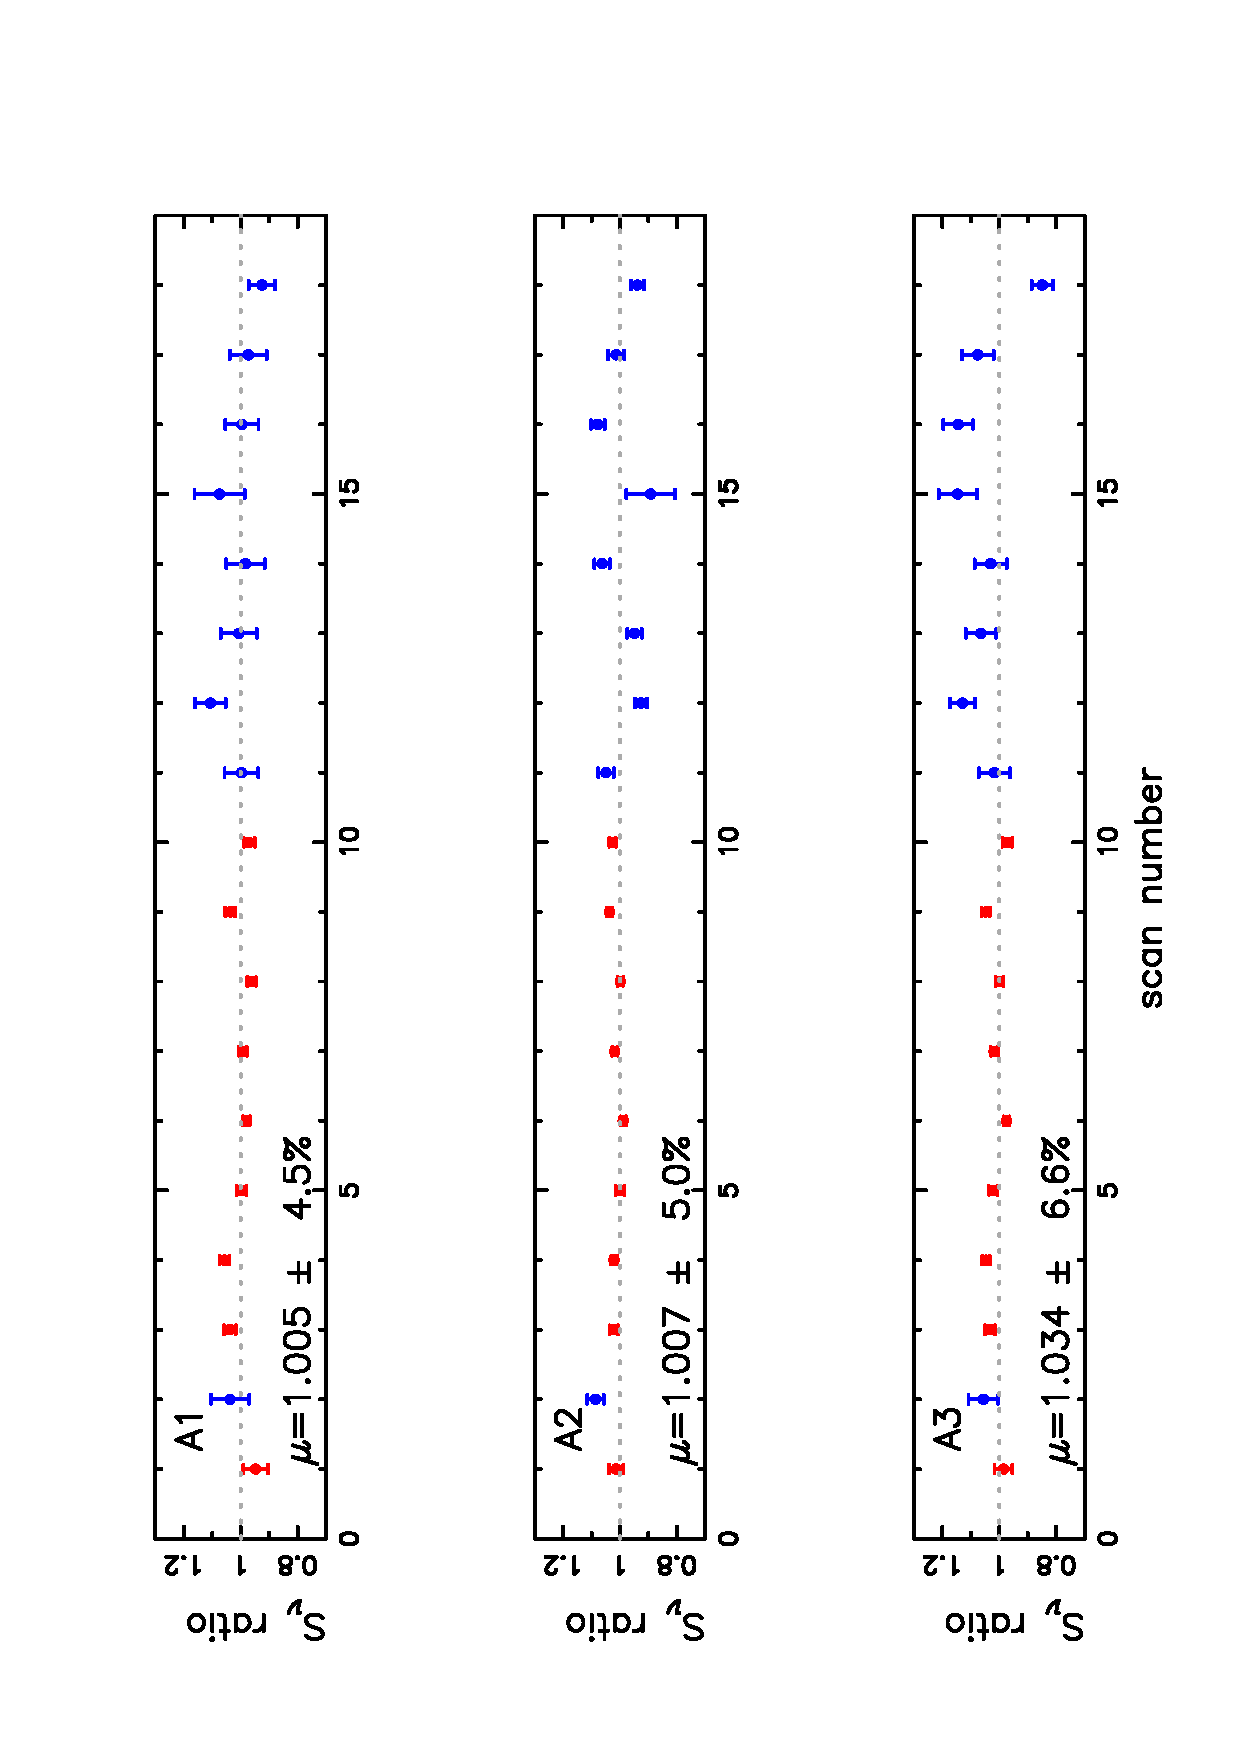
\includegraphics[clip, angle=-90, scale=0.6]{Figures/Ura_Nept_r9_10.pdf}
  \caption{Stability of calibration with the primary calibrators
    Uranus (red) and Neptune (blue)  shown in plotting
    ratios between their measured and reference flux densities during run 9 and 10.
    Mean ratio $\mu$ and scatter in percent are provided for each array.
    Observation numbers are time ordered : 1 to 10 are during run 9 (23-28 february 2017) and 11 to 18 are during run 10 (19-25 april 2017).
    Neptune was hardly visible at the telescope during run 9, and Uranus was not visible during run 10.
    Observations are beammaps (22 min) and integrated sequence of 4 consecutive 4 minute long otfs (16 min) that are
    comparable in integration times.}
\label{fig:U_N_ratio}
\end{center}
\end{figure}

\begin{figure}[p]
\begin{center}
  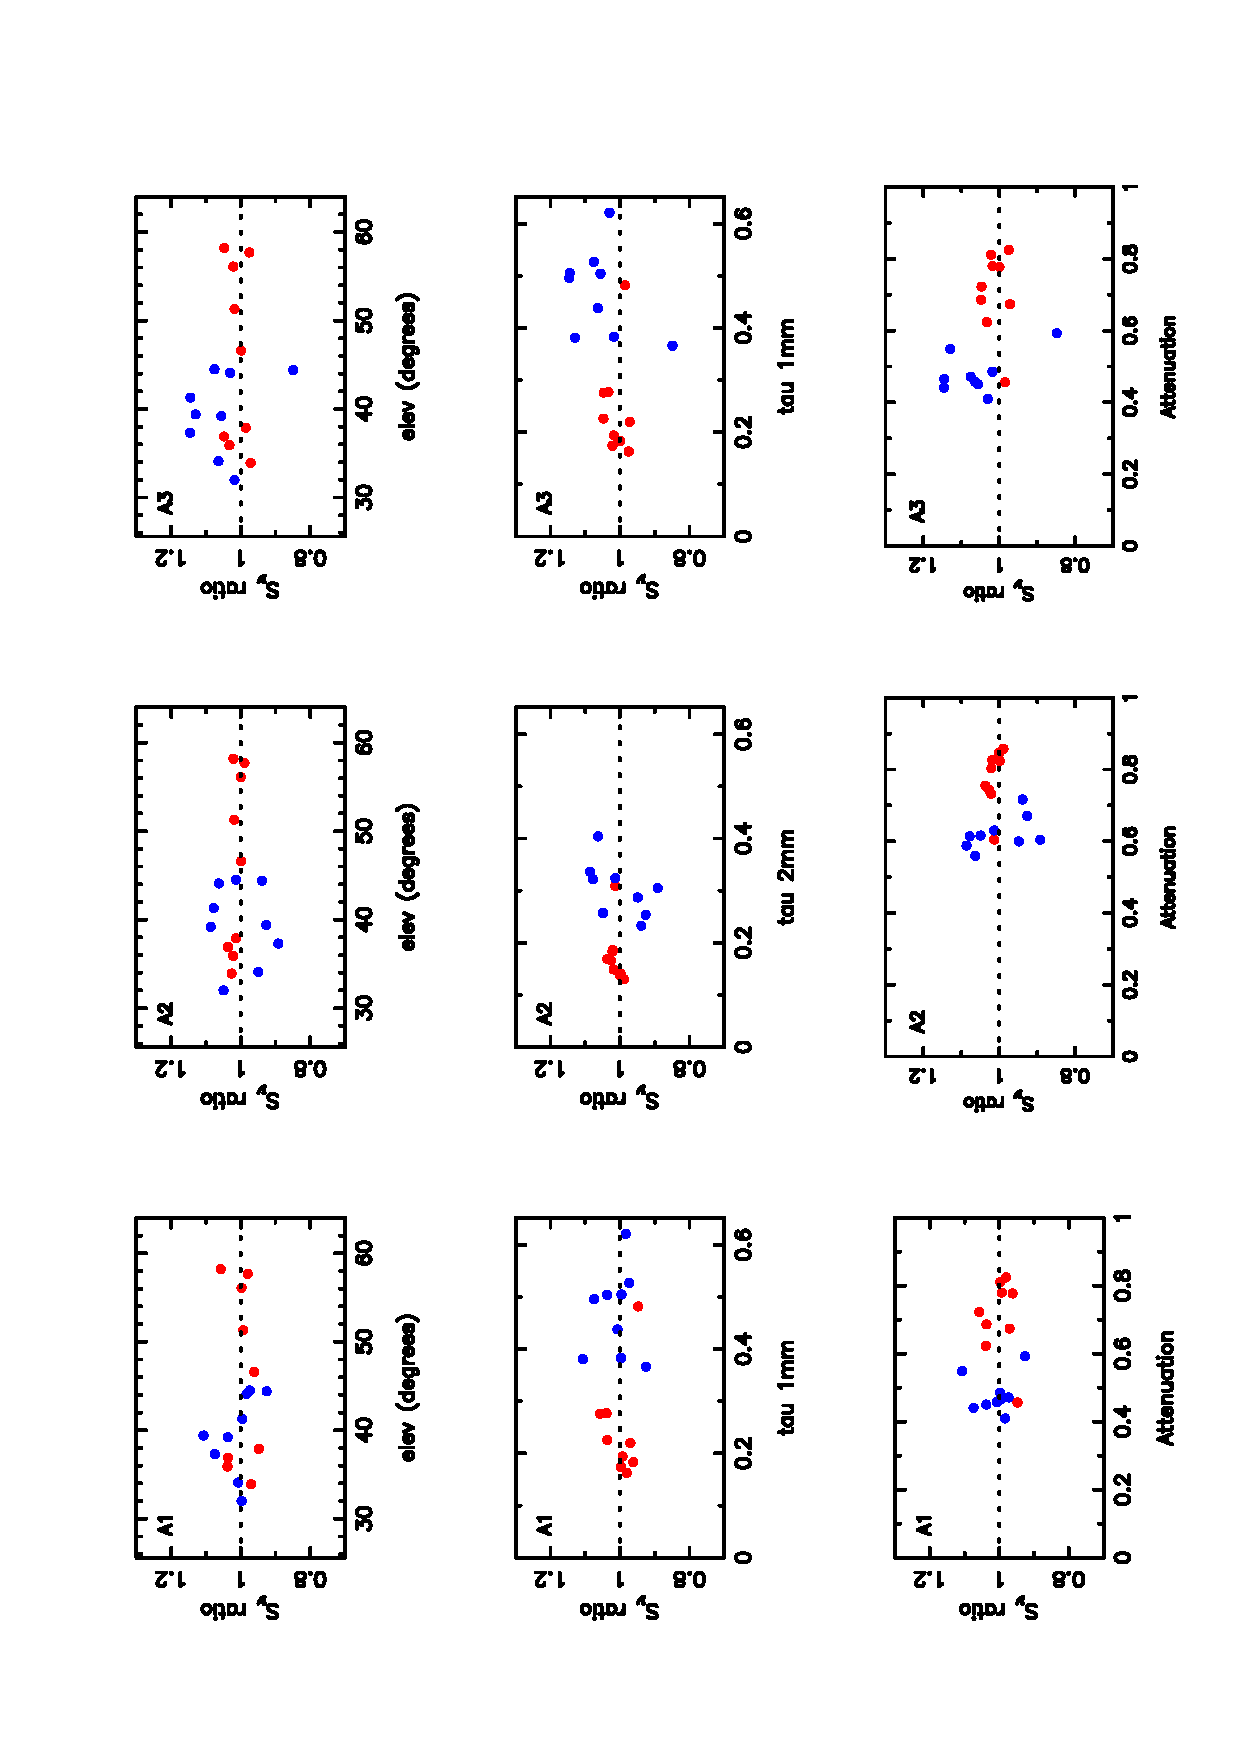
\includegraphics[clip, angle=-90, scale=0.6]{Figures/Ura_Nep_ratio_vs_elev_tau_attenuation_r9_r10.pdf}
  \caption{Flux density ratios versus elevation, opacity, and attenuation ($exp(-\tau/sin(elev)$) for Uranus and Neptune.
    No correlation is apparent with attenuation. {\bf FM: the scale of
      the y axis should be much shorter  ;   JFL's reply  : will be done for final
    version of document}}
\label{fig:ratio_vs_att}
\end{center}
\end{figure}


\begin{figure}[p]
\begin{center}                                                                                                             
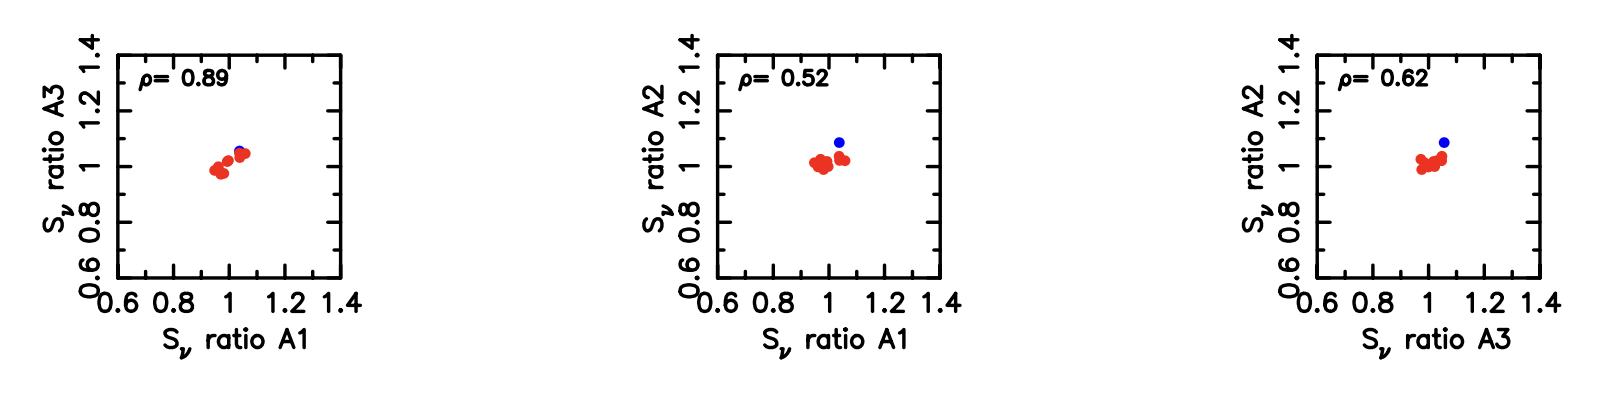
\includegraphics[clip, angle=0, scale=0.55]{Figures/Corr_r9.png}
  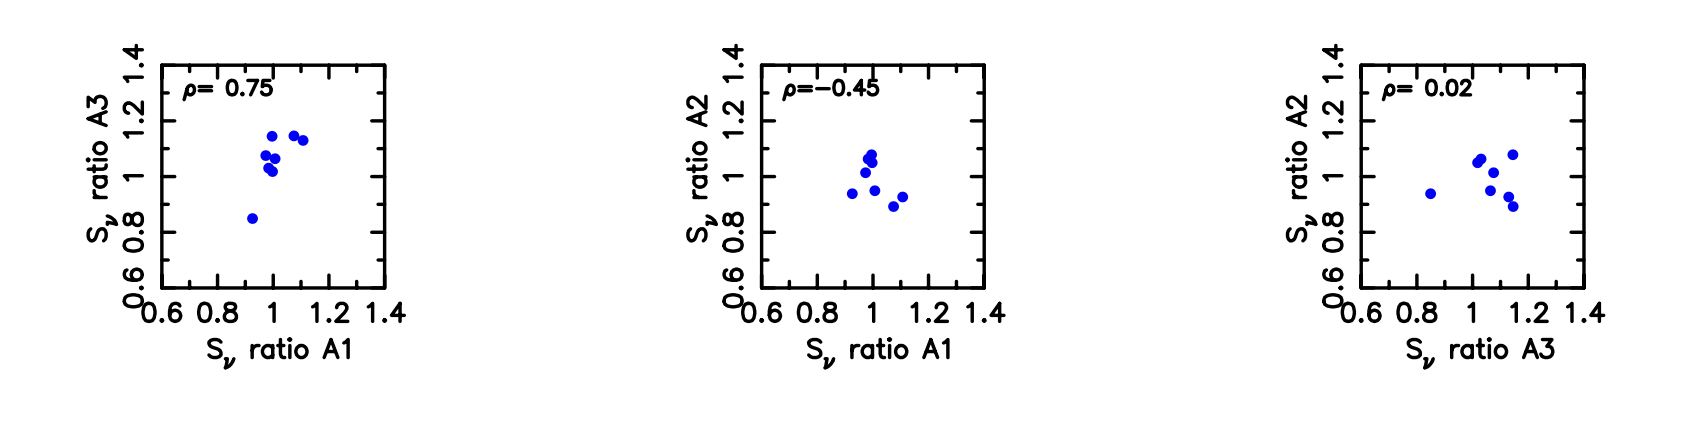
\includegraphics[clip, angle=0, scale=0.55]{Figures/Corr_r10.png}  
  \caption{Correlation plots for the flux density ratios between  the three arrays
    shown separately for run 9 in the first line (fair atmospheric condition),  and for run 10 in second line (mediocre condition).
    Correlation coefficients $\rho$ are given. {\bf FM: the scale of
      the y and x axis should be much shorter ; JFL's : will be done for final
    version of document}}
\label{fig:U_N_corr}
\end{center}                                                                                                             
\end{figure}


\begin{figure}[p]
\begin{center}
  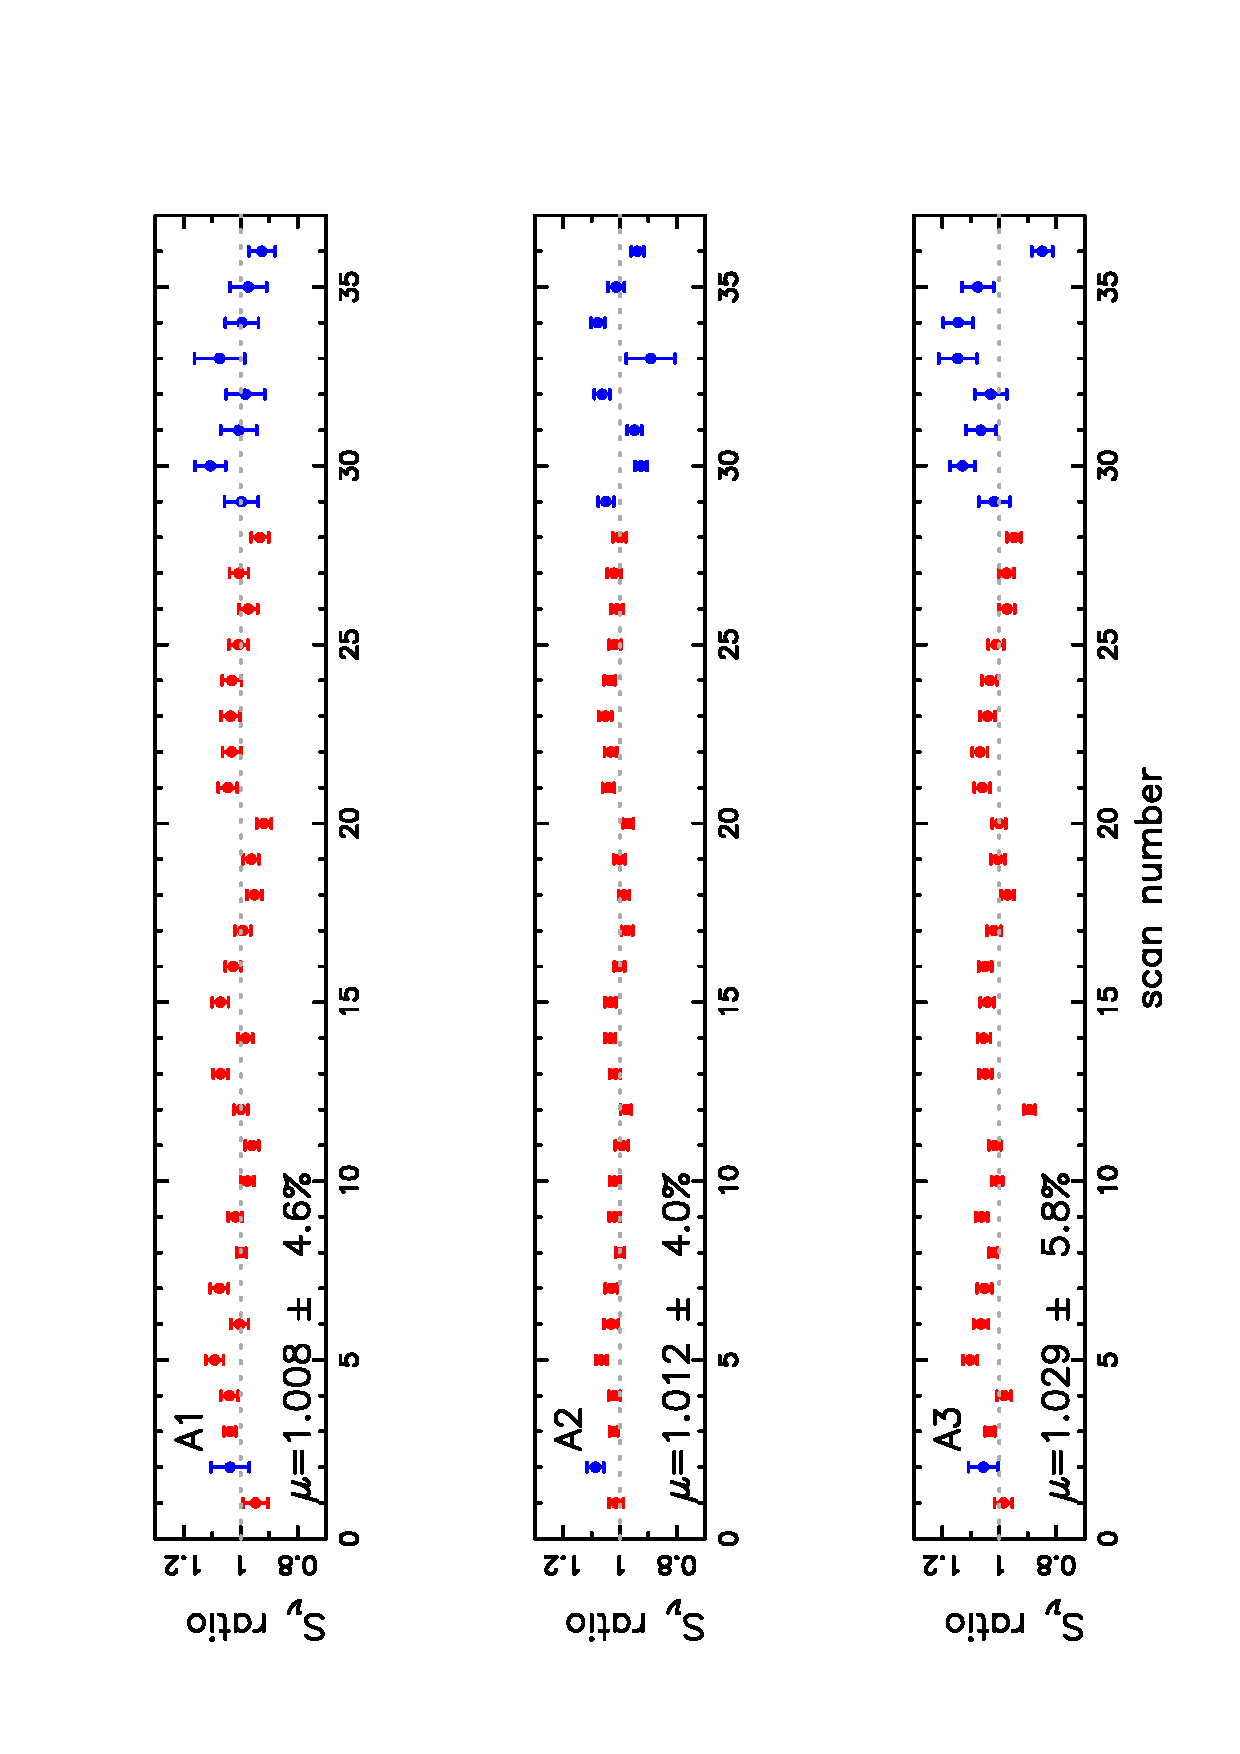
\includegraphics[clip, angle=-90, scale=0.6]{Figures/Flux_ratio_index_A1_A2_A3.pdf}
  \caption{Stability of calibration with the primary calibrators Uranus (red) and Neptune (blue).
    In this plot, single 4 minute long otf's of Uranus acquired during
    run 9 are kept separate, 
while, in Fig.\ref{fig:U_N_ratio} above, observations of 4 consecutive otf's were integrated together (16 min).
    Means and rms of flux density ratios are not significantly different though.}
\label{fig:U_otf_indiv}
\end{center}
\end{figure}

\clearpage
\newpage

\subsection{Calibration of the secondary calibrators MWC349A, NGC7027 and CRL2688}

The sources  MWC349A, NGC7027 and CRL2688 are standard secondary calibrators
and were observed during runs N2R9 and N2R10. Their reference flux densities at
the NIKA2  frequencies of 150 and 260 GHz are in
Table~\ref{tab:flux_ref_sec} and were predicted  from the literature for  NGC7027 and CRL2688
(see \S~\ref{se:fluxSec}) and from the IRAM monitoring program at PdB for MWC349A  \cite{krips}.
Thirteen  of the 84 observations (sequence of 4 consecutive 4 min long otf's) of these three secondary calibrators were discarded because
aperture photometry failed.

As for the planets, the observations of these secondary calibrators were processed with the pipeline set up with the parameters
of Table~\ref{tab:Pipe}. In this scheme, the basic conversion from KID Hz shifts to Jy/beam is done through the   
kidpars,  {\it kidpar-best3files-FXDC0C1-GaussPhot} for run 9 and {\it kidpar-n2r10-calib} for run 10, which were calibrated 
with Uranus and Neptune. Maps of the secondary calibrators were produced and their
flux densities  were measured with two methods : aperture photometry in Table~\ref{tab:flux_sec_Ap},
and  the pipeline Gaussian fit in Table~\ref{tab:flux_sec_NK}. For aperture photometry, the solid angle of the total beam $\Omega_{true}$
was determined for each observation, while  for the pipeline Gaussian photometry a fixed solid angle is assumed 
and  based on the reference FWHM $12.5''$ and $18.5''$.
\footnote {Although flux densities  $S_{\nu}$ were measured at 
the central frequencies of the arrays $\nu_c$ (255, 152, 258 GHz) adopted initially for
the kidpars of Table~\ref{tab:Pipe}, they were changed afterward to the NIKA2 reference
frequencies  $\nu_{ref}$  (150, 260GHz) in using  the correction 
$\Delta S_{\nu}  = \alpha S_{\nu} (\nu_{ref}-\nu_c)/\nu_c $) with the spectral indices $\alpha$ 
($S_{\nu} \propto \nu^{\alpha}$) of the calibrators in Table~\ref{tab:flux_ref_sec}. These changes are less than 5\%.}
Color-corrections have been applied
with indices $\alpha=+0.6$, $-0.34$ and $+2.44$ for MWC349A, NGC7027 and CRL2688, respectively, while Uranus and
Neptune have $\alpha=+1.6$. These color corrections are smaller than 2.5\% (see Table in
\S~\ref{se:cal_HA}, CAUTION : this table is pending in  HA section).  
%Again, both of these corrections are included in Tables~\ref{tab:flux_sec_Ap} and \ref{tab:flux_sec_NK} 
%where the flux densities and uncertainties are the mean and rms of all observations of each source during each run. 
Note that in Tables~\ref{tab:flux_sec_Ap} and \ref{tab:flux_sec_NK}, for each calibrator, its
flux density and uncertainty  are  the mean and
standard deviation of all its observations with an array during a run.   
Note again that each observation is the integration of 4 consecutive otf scans (total 16 minutes). 

\begin{table}[th]
\begin{center}
\begin{tabular}{|c|c|c|c|c|c|}
\hline
\multicolumn{3}{|c}{}  & \multicolumn{3}{|c|}{Flux densities (Jy)}   \\
\hline
         & run  & \#obs &  A1                    &  A2                   &    A3                    \\
         &      &      &  $S_{260 {\rm GHz}}$     &  $S_{150 {\rm GHz}}$  & $S_{260 {\rm GHz}}$    \\
\hline\hline
MWC349A   &  9   & 10  &  $2.23\pm0.32$  ($+8.2\%$)  &  $1.49\pm0.11$ ($+0.6\%$) &  $2.15\pm0.35$ ($+4.6\%$)      \\
  $''$   & 10   & 14  &  $1.96\pm0.17$  ($-4.8\%$)  &  $1.48\pm0.08$ ($+0.2\%$) &  $2.10\pm0.19$ ($+1.8\%$)                  \\ 
  \hline
NGC7027  &  9   & 13  &  $3.22\pm0.39$  ($-6.9\%$)  &  $4.19\pm0.18$ ($-1.6\%$) & $3.05\pm0.54$  ($-11.9\%$)      \\
  $''$   & 10   & 15  &  $3.01\pm0.36$  ($-13.0\%$) &  $4.04\pm0.30$ ($-5.2\%$) & $3.31\pm0.19$  ($-4.2\%$)                   \\ 
  \hline
CRL2688  &  9   & 11  &  $2.91\pm0.48$  ($-0.1\%$)  &  $0.59\pm0.05$ ($-22.9\%$)  &  $2.68\pm0.51$ ($-7.9\%$)     \\
  $''$   & 10   &  8  &  $2.36\pm0.14$  ($-19.0\%$) &  $0.52\pm0.04$ ($-32.1\%$)  &  $2.49\pm0.18$ ($-14.5\%$)                   \\
\hline
\end{tabular}
\caption{Flux densities from {\bf aperture photometry} and relative differences   with respect to reference values.}
\label{tab:flux_sec_Ap}
\end{center}
\end{table}
%open(1,file='sequence_Ur_Nep_r_8_9_10.dat' (contient aussi cal sec du r 9 seulement)  ;  flux=flux
% open(1,file='run10_cal_sec.dat')    ! kidpar_n2r10_calib (mask=50") with F2D, bramax (seul fichier avec cela)    
% cahier II p. 46, 47 : corrections (255, 258GHz) --> 260GHz  (152GHz) --> 150GHz  and color-correction with Table p.37

\begin{table}[bh]
\begin{center}
\begin{tabular}{|c|c|c|c|c|c|}
\hline
\multicolumn{3}{|c}{}  & \multicolumn{3}{|c|}{Flux  densities (Jy)}   \\
\hline\hline
         & run  & \#obs &  A1                        &  A2                        &           A3                  \\
         &      &       &  $S_{260 {\rm GHz}}$       &  $S_{150 {\rm GHz}}$       & $S_{260 {\rm GHz}}$         \\
\hline  
MWC349   &  9   & 10    &  $1.98\pm0.16$ ($-4.1\%$)  &  $1.46\pm0.05$ ($-1.3\%$)  &  $2.02\pm0.17$ ($-2.0\%$)     \\
  $''$   & 10   & 14    &  $1.71\pm0.16$ ($-16.8\%$) & $1.44\pm0.05$ ($-2.5\%$)   &  $1.84\pm0.20$ ($-10.7\%$)      \\ 
  \hline
NGC7027  &  9   & 13    &  $3.53\pm0.33$ ($+2.1\%$)  &  $4.28\pm0.18$ ($+0.4\%$)  & $3.62\pm0.36$ ($+4.7\%$)      \\
  $''$   & 10   & 15    &  $3.27\pm0.19$ ($-5.5\%$)  & $4.28\pm0.14$ ($+0.6\%$)   &  $3.53\pm0.19$ ($+2.1\%$)        \\ 
  \hline
CRL2688  &  9   & 11    &  $2.53\pm0.23$ ($-17.0\%$) &  $0.55\pm0.02$ ($-27.5\%$) &  $2.49\pm0.24$ ($-14.2\%$)    \\
  $''$   & 10   &  8    &  $2.22\pm0.12$ ($-23.6\%$) &  $0.54\pm0.02$ ($-29.3\%$) &  $2.32\pm0.13$ ($-20.4\%$)     \\
\hline
\end{tabular}
\caption{Flux densities  from {\bf pipeline} gaussian fit and relative differences  with respect to reference values.}
\label{tab:flux_sec_NK}
\end{center}
\end{table}
%open(1,file='sequence_Ur_Nep_r_8_9_10.dat' (contient aussi cal sec du run 9 seulement) ;   flux=S_NK
% open(1,file='run10_cal_sec.dat')    ! kidpar_n2r10_calib (mask=50") with F2D, bramax (seul fichier avec cela) 

\noindent {\bf FM: i'm not sure that the relative differences with respect to reference values is an interesting parameters as in our case 
the bias, if any, is small than the error bars.}\\

\noindent {\bf FM: I think it would help the reader to have the values of these tables on a figure (or 2) to judge by eye is there is an
agreement. Moreover, the comparison requires to use a table given 10 pages before. The assessment of the photometry is a key point that would deserve an illustration. (but keep the tables as well}\\

\noindent {\bf JFL reply to FM : OK, in a short while, I will make a plot to summarize  the two tables and will remove \% differences
  from Tables (but they are kept in in the meantimes}\\

By inspection of Tables~\ref{tab:flux_sec_Ap} and \ref{tab:flux_sec_NK}, we conclude that :

\begin{itemize}
  
\item measured flux densities are statistically consistent when results are compared between runs 9 and 10 despite very different weather conditions.
Satisfactorily, this is an indication that the atmospheric signal is properly removed from the raw data by the pipeline.   


\item   measured flux densities are biased at the  10\% level when results are compared between the two methods
(aperture photometry and pipeline Gaussian photometry) ;
for each calibrator,  it is 10\% up for MWC349A and CRL2688 (point sources) while it is 10\% down
for NGC7027 (slightly extended) and it is similar for the three arrays.
This bias between the two methods should be investigated further but it indicates
already that the two methods are viable. We remind that the
pipeline fits the source with a Gaussian with a reference FWHM empirically fixed to $12.5''$ or $18.5''$, {\it i.e.} larger than the main beam width
in order to approximate the complexe profile of the beam.  

\item measured flux densities of MWC349A and NGC7027 are statistically consistent when compared to the reference flux densities of
Table~\ref{tab:flux_ref_sec}. This is not true
     for CRL2688 which is found to be 20\% lower at 1mm and 30\% lower at 2mm. This overestimation of the reference flux densities
      in Table~\ref{tab:flux_ref_sec}   is likely due to the large lever arm in frequency when extrapolating from
      the SCUBA2 850 $\mu$m (345 GHz) and 450 $\mu$m (650 GHz) measurements to the NIKA2 frequencies 150 and 260~GHz,
      and because of the large uncertainty of  the SCUBA2 450 $\mu$m flux density.
      However, we note again that the NIKA2 flux densities of CRL2688 are satistically consistent between the two runs.
      Future measurements should be planned
      for confirmation of this stability before CRL2688 is considered a reliable calibrator.

\end{itemize}

Finally, we provide the ratios between measured and reference flux densities for MWC349 only because
its reference flux densities are monitored at PdB
       by Iram at frequencies close to NIKA2 and so are the most reliable among the three secondary calibrators.
       Ratios are given for aperture photometry in Fig.~\ref{fig:ratio_349_Ap}, and  given for
       the pipeline Gaussian photometry in Fig.~\ref{fig:ratio_349_NK}.
       The mean ratio and rms are provided in the figures. At 1mm, rms  are $\sim$~10\% on arrays A1 and A3 
       and are slightly better
       in using the pipeline Gaussian photometry than aperture photometry.
       However, for the  pipeline Gaussian photometry, the mean ratios are systematically lower than unity by $\sim$~10\% at 1mm.
        This bias in using the pipeline Gaussian photometry
       is also found for the Uranus and Neptune data of runs 9 and 10 but at a level of 5\% at both bands. It is likely that an adjustement
       of the reference FWHMs for the pipeline Gaussian fit (currently $12.5''$ and $18.5''$) could remove this bias.


\subsection{Gain-elevation curve}


We have searched for any elevation dependence of the solid angle of the total beam  $\Omega_{true}$ of Uranus and Neptune
and found none for
the elevation range of their observations between  30$^{\circ}$ and 65$^{\circ}$.  We have also studied such a dependence
for the observations of the three secondary calibrators which span a larger range between elevations 23$^{\circ}$ and 74$^{\circ}$.
The most conclusive study is for NGC7027, the brightest secondary calibrator, in Figure~\ref{fig:gain_curve_NG7027}. 
Its pipeline Gaussian photometry exhibits some degree of curvature centered around elevation 45$^{\circ}$ and in a similar way
for the three arrays.
While the pipeline Gaussian photometry  assumes a fixed solid angle for the total beam based on the reference FWHM's $12.5''$ and $18.5''$,
the solid angle as determined with the data themselves in using
eq.~\ref{eq:Otrue} exhibits instead a similar curvature centered on elevation 45$^{\circ}$. This needs confirmation with further
observations  over the largest elevation range possible at the telescope and on the strongest source available. Note finally,
that the flux density of NGC7027 determined
with aperture photometry does not exhibit any curvature, as expected, since the conversion factor ${dx^2} \over {\Omega_{true}}$
in eq~\ref{eq:ApPh} models the effect.  We stress again that the EMIR gain curved was not turned on to process the data. 





%From these two tables, we conclude that  the 2 mm flux densities of MWC349A and NGC7027 measured with array 2 are consistent with predictions,
%and consistent between runs (9 and 10) and methods (aperture photometry, pipeline Gaussian fit) at the few percent level
%($(S_{meas}-S_{ref})/S_{ref} \times 100)$. But this is not the case for CRL2688.  Its NIKA2 2mm
%flux density is $\sim$25\% lower than prediction, consistently between runs and methods. Hence, this may be due to an over estimation
%in the prediction of the 2 mm flux density that was extrapolated from the SCUBA2 850 $\mu$m and 450 $\mu$m measurements
%and because of the large lever arm in frequency. We note this
%over estimation seems to be also true at 1mm for this source in the two Tables.
%Future observations of CRL2688 will check wether or not its new NIKA2 flux densities are valid to populate usefully its SED
%for science purpose. {\bf FM : so the conclusion is that it is not a reliable calibrator and we should not use it hereafter}

%For the 1 mm flux densities of MWC349 and NGC7027 from these two tables, we conclude that their  measurements with arrays 1 and 3 are
%at the 10\% level   ($(S_{meas}-S_{ref})/S_{ref} \times 100)$  and are consistent with statistical uncertainties estimated from
%the rms of their fluctuations
%during the two runs and shown in Fig.~\ref{fig:ratio_cal_sec}. 


%{\bf FM: {\it at the 10\% level} was said to be {\it the few percent level} a few lines above.}\\

%{\bf FM: i would suggest to remove CRL2688 from Fig.~\ref{fig:ratio_cal_sec}. From the discussion of the text we conclude that it can not be used for calibration as the
%    flux at 1 and 2 mm my be biased due to the extrapolation. This way we can conclude from the figure that NIKA2 photometry is at the 10\%
%    level.}\\
    
%    {\bf FM: i would suggest to change the scale in Fig.~\ref{fig:ratio_cal_sec} as we want to show a 10\% effect...}\\
    
%    {\bf FM: for Fig.~\ref{fig:ratio_cal_sec} histograms would be a better choice as we want to evaluate by eye, the rms, the agreement
%    with one of this ratio of values. Moreover, effect of  weather conditions (tau) is shown on fig. \ref{fig:corr_cal_sec}}\\

%For example, NGC7027, A1, run 10, aperture photometry in Table~\ref{tab:flux_sec_Ap}
%yields  :

%$$rms(S_{obs})/<S_{obs}>=0.36Jy/3.01Jy \times 100=11.9\%$$

%\noindent which is statistically consistent with :

%$$|(S_{meas}-S_{ref})/S_{ref}| \times 100=15.0\%~,$$

%\noindent where $S_{meas} = <S_{obs}>$.

%Finally, we have plotted the flux density ratios versus elevation, opacity and attenuation  for three
%secondary calibrators in  Fig.~\ref{fig:corr_cal_sec}. No clear correlation is apparent.


%{\bf FM: you should say whether pipeline or aperture value is used for the ratio}\\


%{\bf FM: by the way, a conclusion on pipeline versus aperture values would be useful regarding future use of the pipeline. (no need to
%perform aperture evaluation ?)}\\


\begin{figure}[p]
\begin{center}
  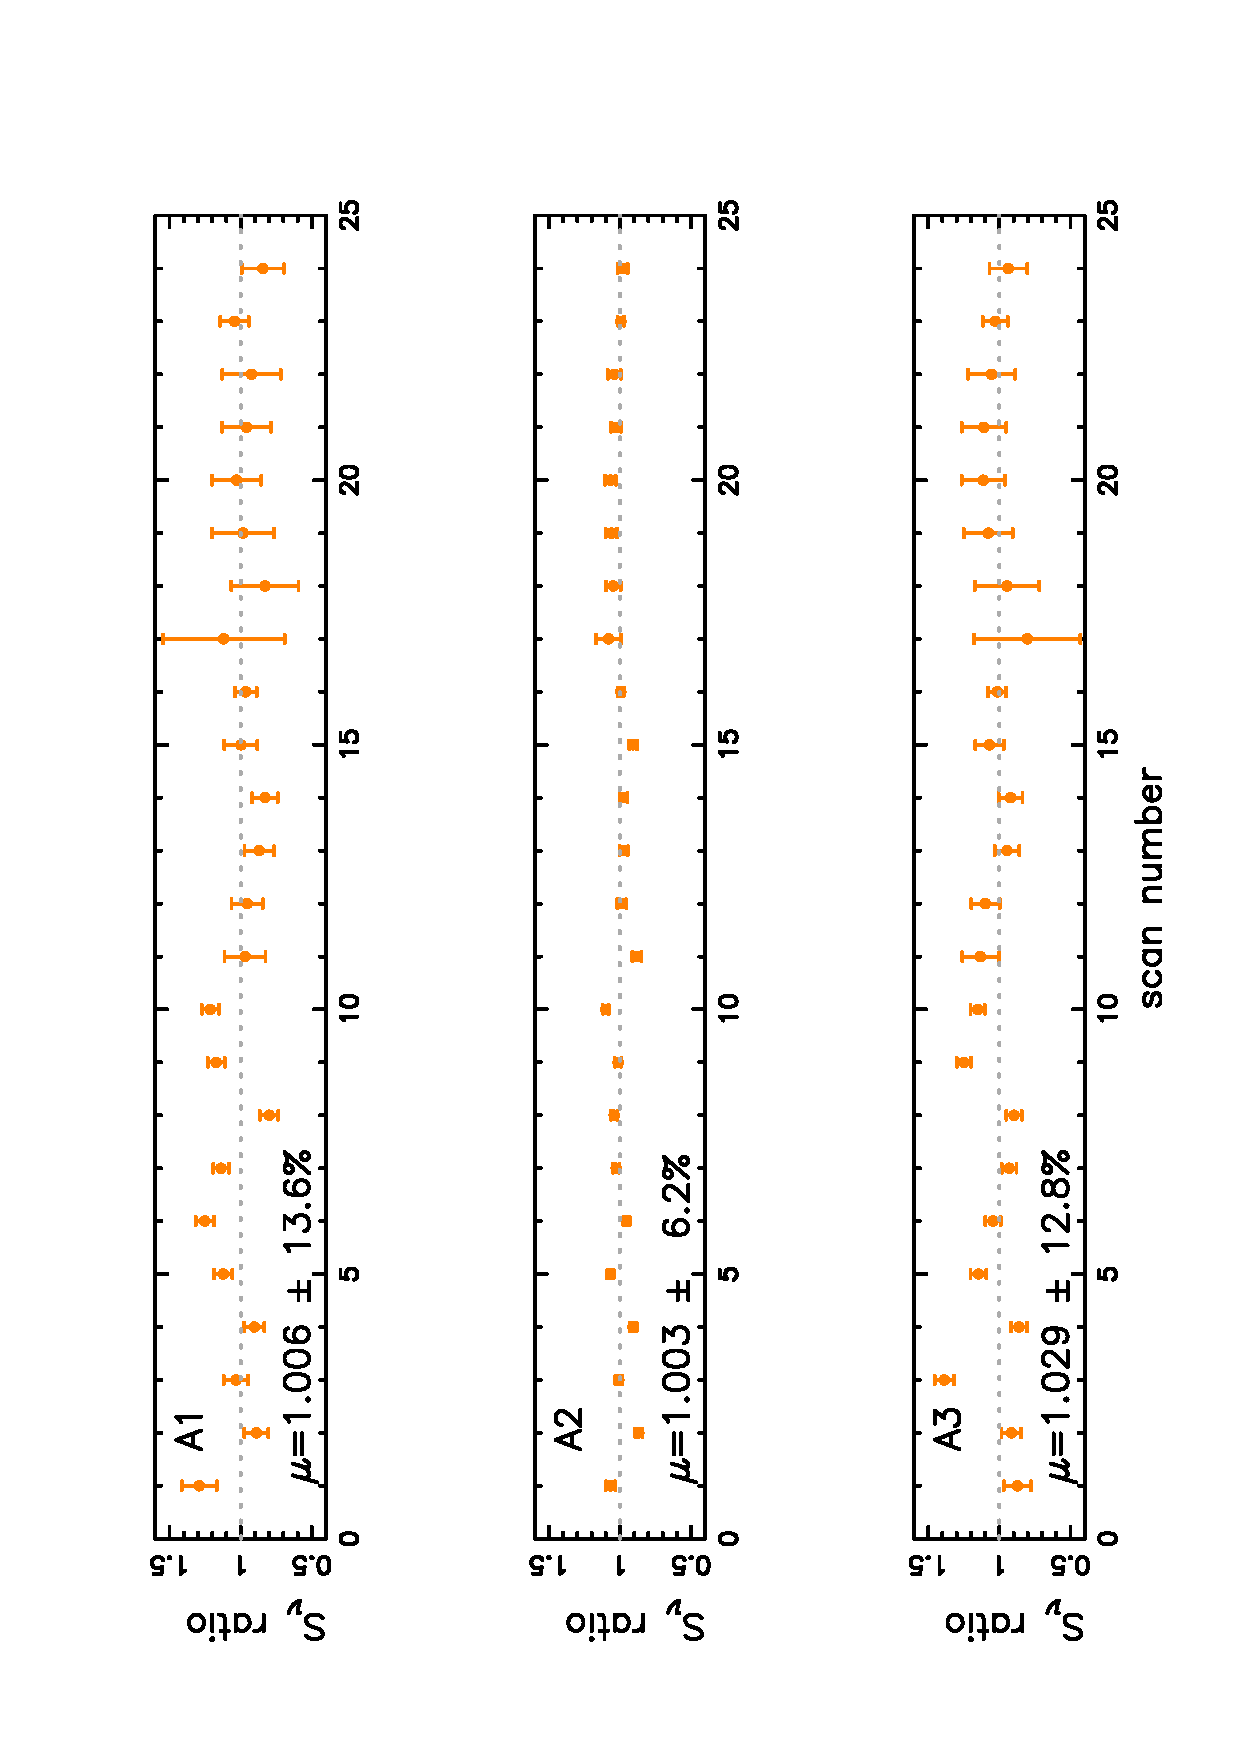
\includegraphics[clip, angle=-90, scale=0.6]{Figures/Ratio_vs_index_MWC349_r9_r10_Ap.pdf}
  \caption{Ratios between measured and reference flux densities of  the secondary calibrator  MWC349A
    during runs 9 and 10.  {\bf The flux density is measured with aperture photometry}. Note that mean ratios
    on the three arrays are close to unity as expected for proper calibration.
    Scan numbers are time ordered (index 1 to 11 : run 9 (fair weather) and index 12 to 24 : run 10 (mediocre weather).
    Each observation is a sequence of 4 consecutive 4 minute long otfs (total integration is 16 minutes).
  }
\label{fig:ratio_349_Ap}
\end{center}
\end{figure}



\begin{figure}[p]
\begin{center}
  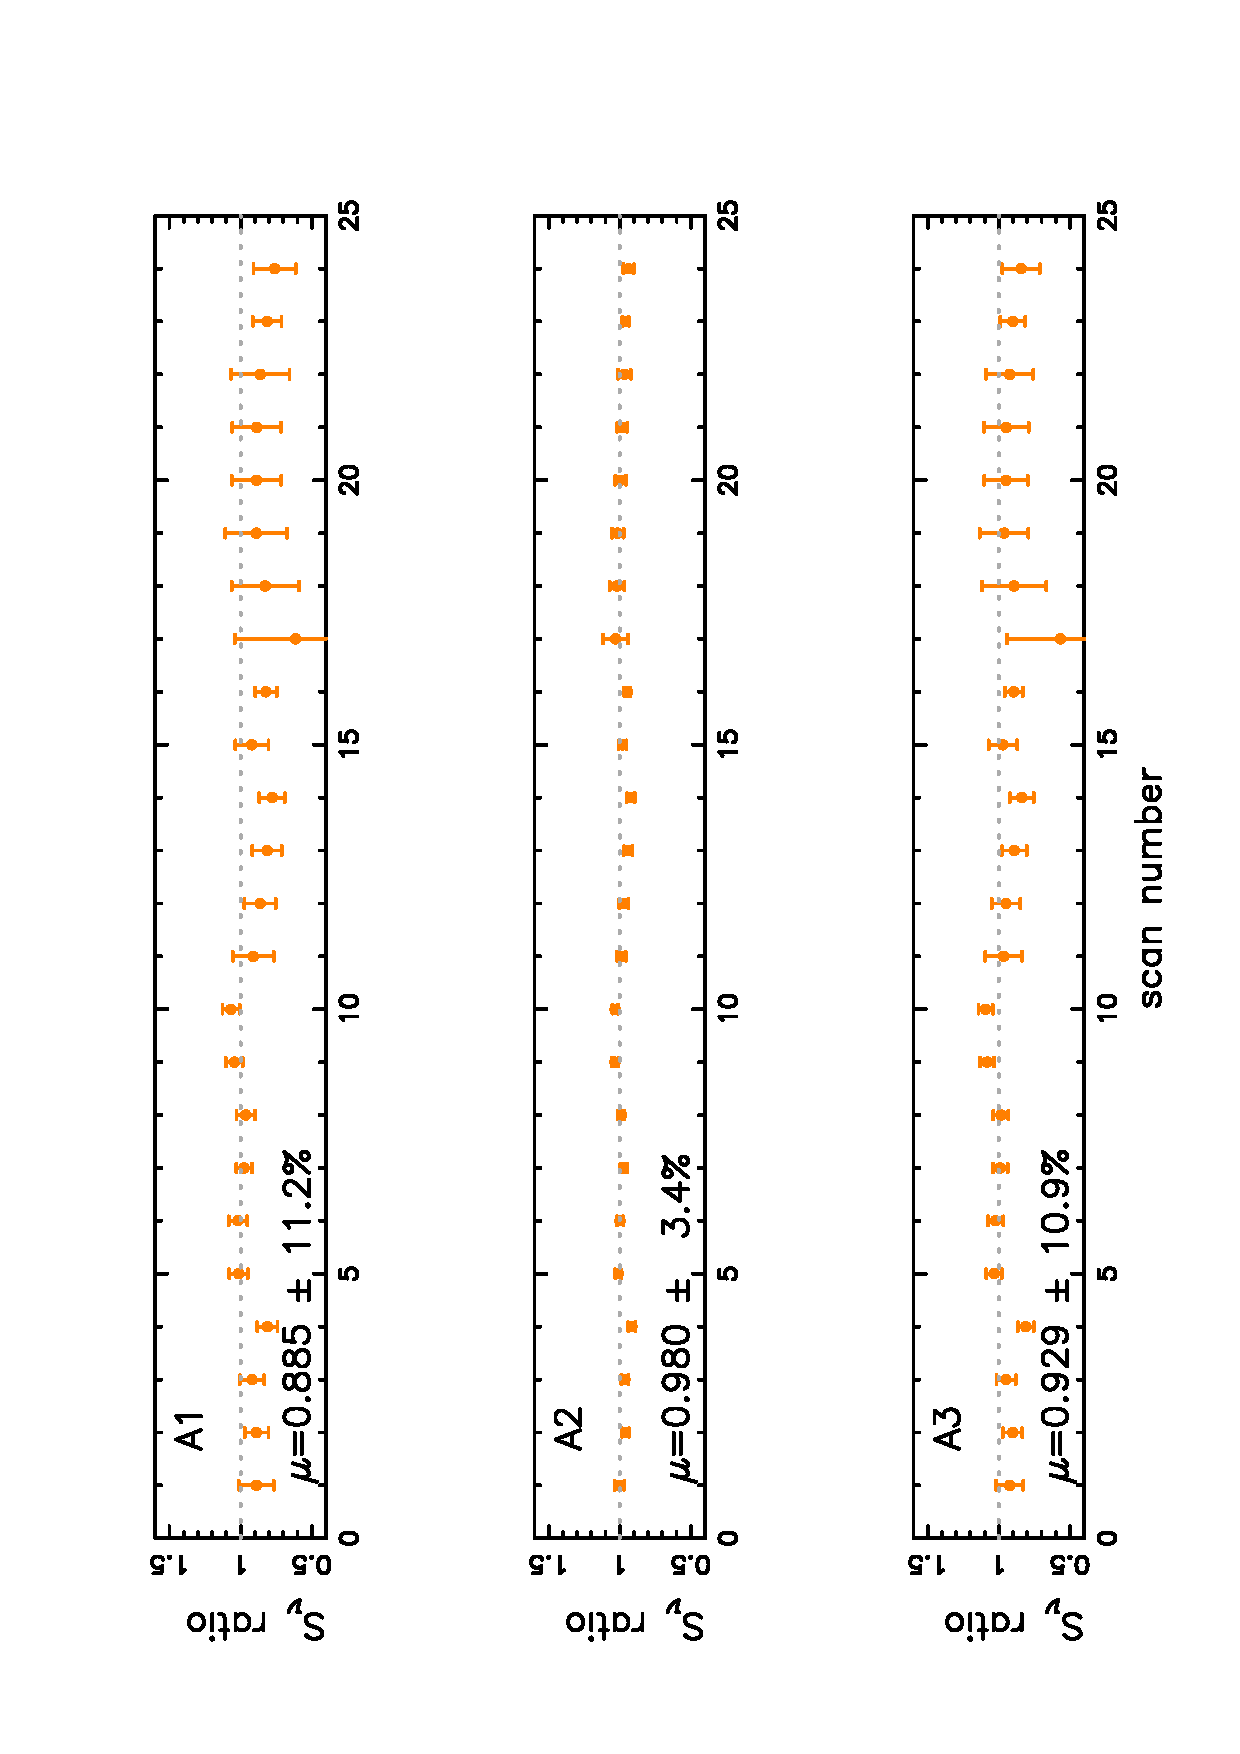
\includegraphics[clip, angle=-90, scale=0.6]{Figures/Ratio_vs_index_MWC349_r9_r10_NK.pdf}
  \caption{Ratios between measured and reference flux densities of  the secondary calibrator  MWC349A 
    during runs 9 and 10.  {\bf The flux density is measured with the Pipeline Gaussian photometry}. Note that mean ratios 
    on A1 and A3 are $\sim$~10 \% lower than unity, unsatisfactorily.
    Scan numbers are time ordered (index 1 to 11 : run 9 (fair weather), and index 12 to 24 : run 10 (mediocre weather).
    Each observation is a sequence of 4 consecutive 4 minute long otfs (total integration is 16 minutes).
  }
\label{fig:ratio_349_NK}
\end{center}
\end{figure}



\begin{figure}[p]
\begin{center}
  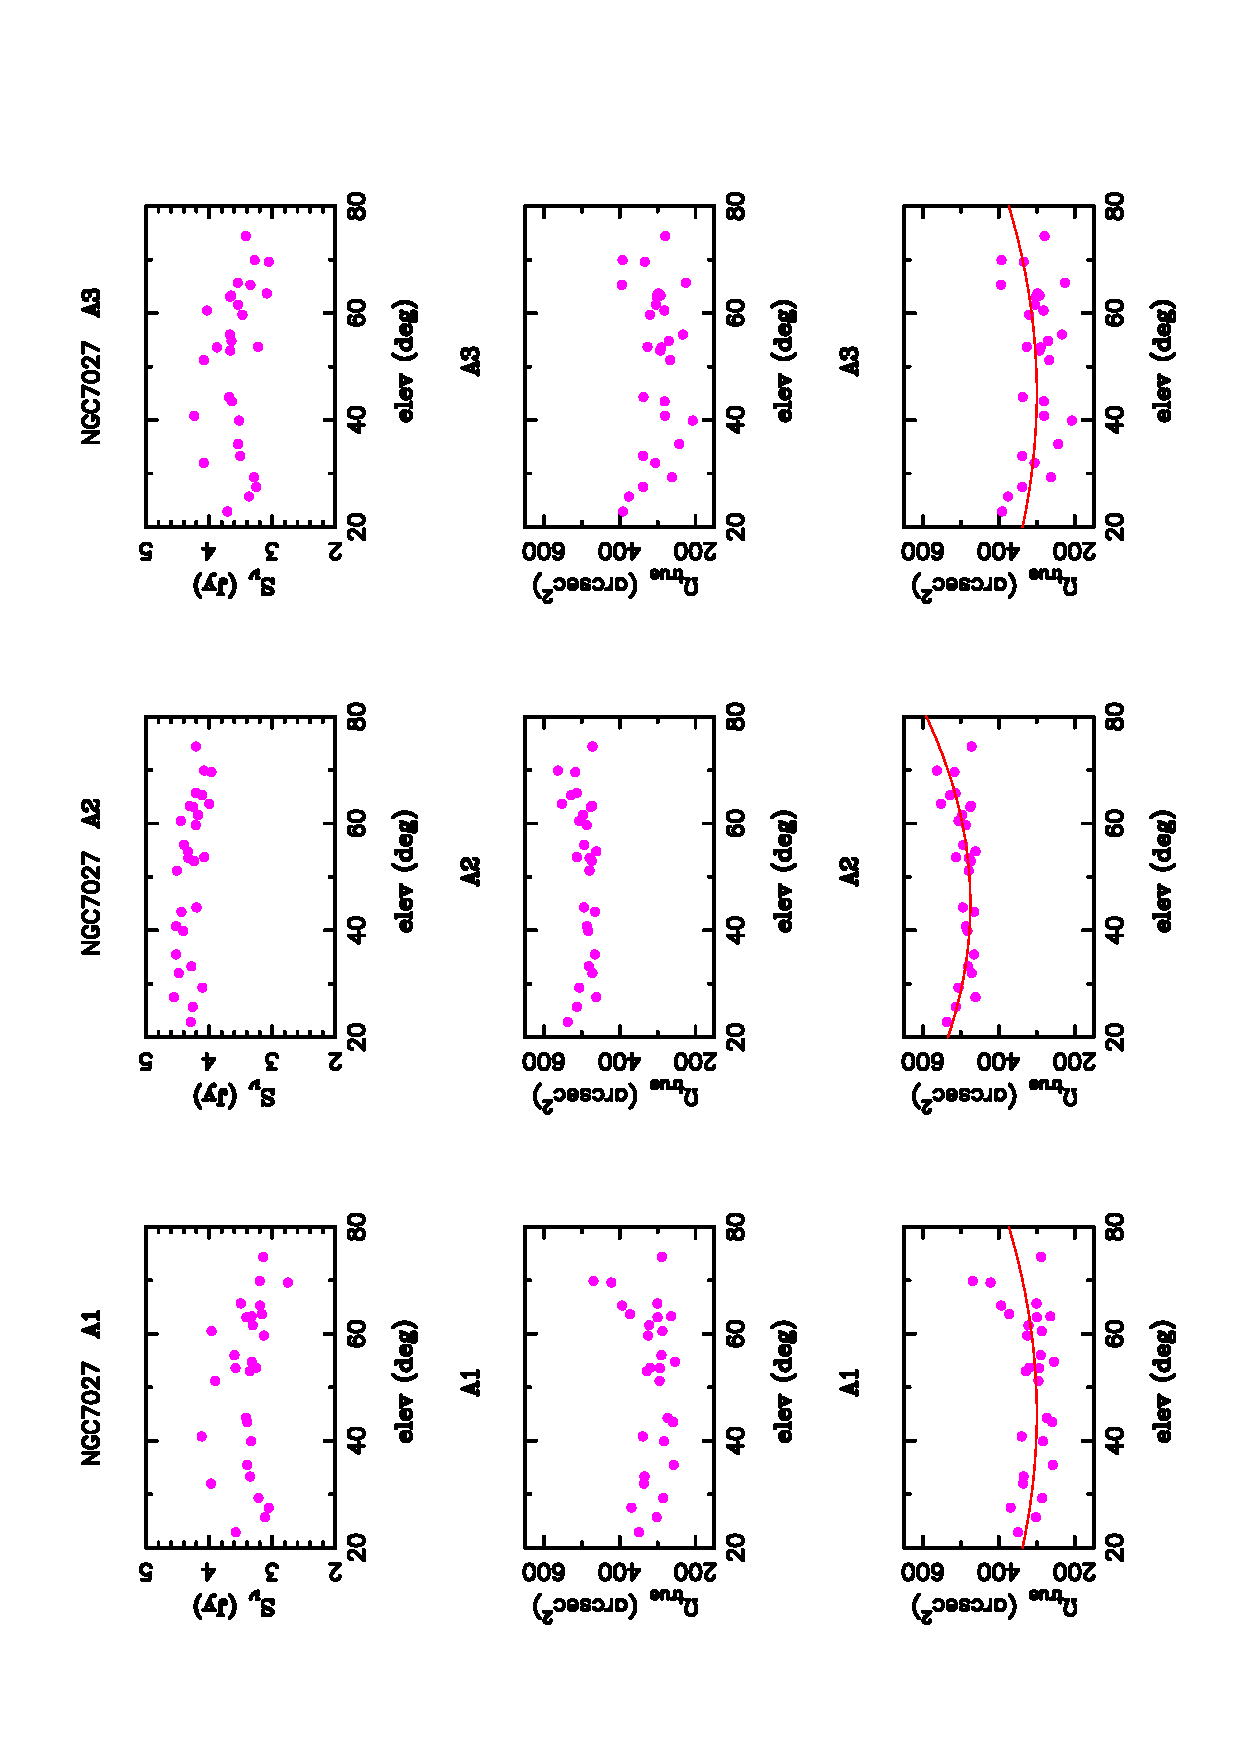
\includegraphics[clip, angle=-90, scale=0.6]{Figures/Flux_gain_curve_NGC7027}
  \caption{{\bf Top line :} Flux densities of the secondary calibrator NGC720 {\bf measured with the pipeline Gaussian photometry}
    with a fixed solid angle
    for the total beam of the telescope. The flux densities are given for the three arrays during runs 9 and 10  and  
    exhibit some degree of curvature over the elevation range of the observations.
    {\bf Second and third lines :} The solid angle of the total beam determined with the observations of NGC7027 themselves. $\Omega_{true}$
    is shown twice ; 
    as  unmarked plots on the second line and with  a ``fit by eye''  centered on  elevation 45$^{\circ}$ on the third line.
    Were this gain-elevation curve applied, it  would flatten the flux density above.  
    Scan numbers are time ordered (index 1 to 13 : run 9 (fair weather), and index 14 to 28 : run 10 (mediocre weather).
    Each observation is a sequence of 4 consecutive 4 minute long otfs (total integration is 16 minutes).
}

\label{fig:gain_curve_NG7027}
\end{center}
\end{figure}


















